\todo{parler également de l'accélération}

Pour pouvoir proposer de nouvelles fonctionnalités de prévention, il faut optimiser le tableau de bord. Il faut créer des logos communs à tous pour avoir le même langage. 

\todo{ajout d'un tableau de bord connecté avec des capteurs et des alertes en temps réel.}
L'idée serait d'intégrer dans les motos une puce GPS qui serait capable d'avertir en cas de virage dangeureux. L'alerte (sonore via un intercom et voyant au tableau de bord) serait envoyée via le tableau de bord connecté si la vitesse est supérieure à la vitesse recommandée. Cette vitesse sera calculée via la valeur de la courbure du virage. Des chercheurs Alex Liniger et Simon Hecker ont développé un prototype , Aegis Rider AG\cite{vitesse_virage_mcnews} permettant de prendre la meilleure trajectoire. Cependant, ce dernier ne prend pas en compte les autres facteurs de la route (autres usagers, état de la chaussée, etc.). Comme démontré ci-dessous, la trace bleu indiquant la trajectoire de sécurité et le compteur de vitesse masquent la qualité de la route par conséquent, le motard ne pourra pas anticiper les dangers de la route (gravillon, trous, ....). À l'heure d'aujourd'hui, cette solution reste extrêmement complexe. Ma solution permettra de fonctionner dans la pluspart des cas.

\begin{figure}[h]
    \centering
    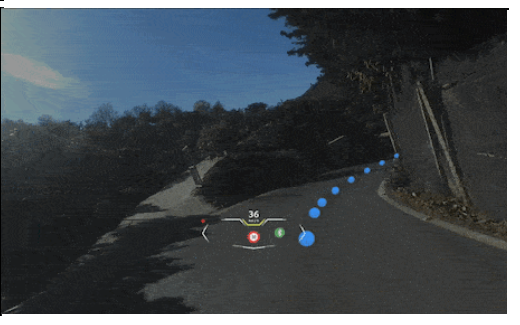
\includegraphics[width=0.7\textwidth]{coeur_memoire/images/aegis.png} 
    \caption{Prototype Aegis Rider AG pour la détection de virages dangereux.}
\end{figure}
Cette fonctionnalité est très interessante mais elle empêche une bonne visibilité de la surface de la route et elle peut fausser une prise de décision.
Comme illustré dans la Figure~\ref{fig:trajectoire_securite_difficulte}, le processus ne pourra pas adapter sur des virages dit "imparfaits".


\todo{voir pour faire une petite ligne de code ?}

\underline{Contexte:} En balade dans le 77, un motard roule sur une départementale. Dans cette situation, il est équipé d'un boitié GPS qui récupère ses coordonnées en temps réel. Il arrive dans une portion de virages limitée à 70 km/h nommée "Les 17 virages", près d'Arbonne-La-Forêt. Cette série de virages est dangeureuse car la route n'est pas bonne, n'est pas large et l'adhérence n'est pas optimale. De plus, il y a un virage dangereux à l'équerre qui surgit au milieu de cette série. La trajectoire de sécurité est fortement recommandé. Par expérience, avoisiner les 70 km/h est déjà bien au vue de la portion qui y est technique.

\begin{figure}[H]
    \centering
    \includegraphics[width=0.7\textwidth]{coeur_memoire/schéma/Capture d’écran 2025-07-24 à 15.45.48.png} 
    \caption{Point GPS des 17 virages.}
\end{figure}

\todo{photo des 17 virages}



Les coordnnées GPS sont : 48.385171, 2.563108.

\todo{mettre le diagramme}
Voici le diagramme d'action de cette fonctionnalité:\\

\begin{figure}[H]
    \centering
    \includegraphics[width=0.8\textwidth]{coeur_memoire/schéma/Capture d’écran 2025-07-24 à 17.48.10.png} 
    \caption{Diagramme d'action du Système de prévention de virages dangereux}
\end{figure}

Pour réaliser un bout de code sur cette fonctionnalité, j'ai décidé d'utiliser ces bibliothèques :\\
• osmnx\cite{osm_doc} : permet d’interroger OSM (OpenStreetMap) et de récupérer des graphes routiers.\\
•	geodesic (de geopy \cite{geopy}) : mesure la distance réelle (en mètres) entre 2 points GPS.\\

L'interêt de calculer la courbure de la courbe est de pouvoir anticiper le virage et par conséquent, adapter la vitesse pour optimiser l'adhérence, la trajectoire où l'on se sentira le plus en sécurité. \\
Le calcul de la courbure permettra d'identifier un virage s'il est dangereux à partir de données GPS cartographiques pour enfin adapter le comportement du système embarqué (alerte, adaptation de trajectoire, assistance..).
Donc la courbure mesure à quel point une route peut changer de direction sur une courte distance, ici, dans un virage.\\
Une route droite a une courbure environ égale à 0. Une route qui tourne fort (virage serré) a une courbure élevée.

\begin{table}[ht]
\centering
\begin{tabular}{|l|c|c|c|}
\hline
Route & Rayon du virage & Courbure (simplifiée) & Risque \\
\hline
ligne droite & infini & 0 & faible \\
Virage large autoroute & 500 m & Faible (0.01) & faible \\
Virage serré en montagne & 30 m & Forte (0.1–0.2) & Élevé \\
\hline
\end{tabular}
\caption{Exemple en pratique}
\end{table}

Un virage serré avec une courbure > 0.1 est souvent dangereux à +60 km/h, surtout à moto.
Plusieurs études indiquent que les rayons < 50 m sont classés comme virages dangereux pour les motos. À plus de 60 km/h, une moto doit pencher à plus de 35°à 40° dans le virage ce qui augmente énormément le risque de chute, surtout s’il y a du gravier, pluie, vent latéral…
L’estimation “courbure > 0.1 = danger > 60 km/h” est une règle empirique, basée sur des données de sécurité moto reonnues, des normes d'ingénierie routière et des approximations géométriques issues de GPS.


L'avantage d'avoir un calcul automatique et en amont, cela permet de prévenir avant même d'être dans le virage. Il peut remplacer un panneau quand celui-ci n'est pas visible. Elle ne remplace pas une analyse dynamique complète mais elle est suffisante pour alerter automatiquement le pilote ce qui est exactement l’objectif du système.



\begin{tcolorbox}[title=Calcul de la courbure]
Courbure mathématique\cite{formule_curvature} d’un virage:
\[
courbure\_virage = \kappa = \frac{1}{R}
\]
où R est le rayon du virage\\
Forme simplifiée de la courbure basée sur la déviation par rapport à une ligne droite.\\
a, b et c sont trois points dans la courbe.\\
\[
courbure = \left| \frac{a + b - c}{a + b} \right|
\]
a + b = distance réelle parcourue en suivant la route \\
c = distance directe entre le début et la fin (comme si on traçait une corde)
\end{tcolorbox}

\begin{figure}[H]
    \centering
    \includegraphics[width=0.7\textwidth]{coeur_memoire/schéma/Capture d’écran 2025-07-22 à 16.27.35.png} 
    \caption{Schéma présentant une moto avant un virage}
\end{figure}


\todo{illustration, développement}

\todo{Détailler le code et les formules de vitesse}
La vitesse recommandée se calcule grace à la courbure.
\begin{tcolorbox}[title=Vitesse recommandée]
Calcul de la vitesse recommandée :
\[
vitesse_{\text{recommandée}} = \max(20, 80-\text{curvature} \times 200)
\]
Le "20" permet d'éviter une vitesse trop basse. Ici, on la limite à 20 km/h.

\end{tcolorbox}

En dessous de 20km/h, il y a peu d'intêret. Même les plus grosses épingles peuvent se prendre à 20km/h. À cette vitesse, il n'y a pas d'effet gyroscopique\footnote{C'est la capacité (tendance) d'un corps en rotation à maintenir une direction constante de son axe de rotation selon le Larousse.}.
Cependant, j'ai plutôt choisi de m'orienter sur des conditions simples pour catégoriser l'intensité du virage pour y associer une vitesse "maximale" qui peut être utilisée sans danger.\\
Voici comment j'ai classé la valeur de la courbure en fonction de la vitesse idéale: \\
•	< 0.0005 → ligne droite → 80 km/h \\
•	de 0.0005 à 0.002 → léger virage → 60 km/h\\
•	>= 0.002 → virage serré → 30 km/h


\vspace{0.5cm}
Voici le code qui permet de récupérer une localisation GPS (latitude, longitude), qui calcule la valeur de la courbure pour après estimer une vitesse de sécurité.
\lstinputlisting[language=Python]{coeur_memoire/programme1.py}

\begin{figure}[H]
    \centering
    \includegraphics[width=0.6\textwidth]{coeur_memoire/images/Capture d’écran 2025-07-29 à 11.39.00.png} 
    \caption{Réseau routier interprété par le programme pour la postion 48.385171, 2.563108}
\end{figure}

\begin{figure}[H]
    \centering
    \includegraphics[width=0.6\textwidth]{coeur_memoire/images/Capture d’écran 2025-07-28 à 12.07.50.png} 
    \caption{Carte du traceur}
\end{figure}

\todo{résultat}
Suite de la mise en situation réelle. Les passages étudiés ont été réalisé bien avant l'expérience, par conséquent, il n'y a aucune notion de vitesse. Chaques passages ont été faits sur la capacité au moment t de l'usager. Voici un premier passage à 51 km/h.
\begin{figure}[H]
    \centering
    \includegraphics[width=0.6\textwidth]{coeur_memoire/images/Capture d’écran 2025-07-28 à 15.56.58.png} 
    \caption{Premier passage dans Les 17 virages}
\end{figure}

Résultat du premier passage avec le programme :
\begin{figure}[H]
    \centering
    \includegraphics[width=0.6\textwidth]{coeur_memoire/images/Capture d’écran 2025-07-29 à 15.37.32.png} 
    \caption{Premier passage dans Les 17 virages}
\end{figure}

Voici maintenant un second passage réalisé un peu plus vite.
\begin{figure}[H]
    \centering
    \includegraphics[width=0.6\textwidth]{coeur_memoire/images/Capture d’écran 2025-07-28 à 16.35.23.png} 
    \caption{Deuxième passage dans Les 17 virages}
\end{figure}


\begin{figure}[H]
    \centering
    \includegraphics[width=0.6\textwidth]{coeur_memoire/images/Capture d’écran 2025-07-29 à 15.37.58.png} 
    \caption{Deuxième passage dans Les 17 virages}
\end{figure}

Le deuxième passage est réalisé plus rapidemment (sans excès de vitesse), cependant, la vitesse est trop "rapide" et nécessite de meilleures capacités pour le passer. Il faut que le motard soit à un niveau bien intermédiaire. Comme l'objectif du programme est de faire de la prévention, j'ai décidé de baser sur un niveau de débutant. Pour conclure, il y a un message qui apparaît.\\
Prenons un dernier exemple avec un nouvel endroit en ligne droite.
\begin{figure}[H]
    \centering
    \includegraphics[width=0.6\textwidth]{coeur_memoire/images/Capture d’écran 2025-07-29 à 14.33.08.png} 
    \caption{Réseau routier}
\end{figure}
Nous avons comme résultat :
\begin{figure}[H]
    \centering
    \includegraphics[width=0.6\textwidth]{coeur_memoire/images/Capture d’écran 2025-07-29 à 14.32.49.png} 
    \caption{Résultat en ligne droite pour les coordonnées 48.514114, 2.320894}
\end{figure}

L'idée maintenant est de prévenir l'usager d'un logo universel. Évidemment, la disposition sera optimisée pour chaque écran. Nous pouvons également y ajouter un bip sonore, cela évitera de fixer en permanance le tableau de bord.
\begin{figure}[H]
    \centering
    \includegraphics[width=0.6\textwidth]{coeur_memoire/images/Capture d’écran 2025-07-25 à 14.42.42.png} 
    \caption{Génération d'un tableau de bord possible avec l'IA.}
\end{figure}

Il pourrait être interessant de poursuivre le développement sur une action sur les freins afin de ralentir légèrement la moto ou bien empêcher ou couper l'accélération. C'est une piste interessante mais cependant, il faut prendre en concidération plusieurs facteurs : \\
• Ne pas surprendre le motard,\\
• Ne pas dimunuer l'adhérence des pneus,\\
• Ne pas inflencer sur la trajectoire de sécurité, or la vitesse joue un rôle crutial dans la trajectoire.
